\begin{figure}[b]
    \centering
    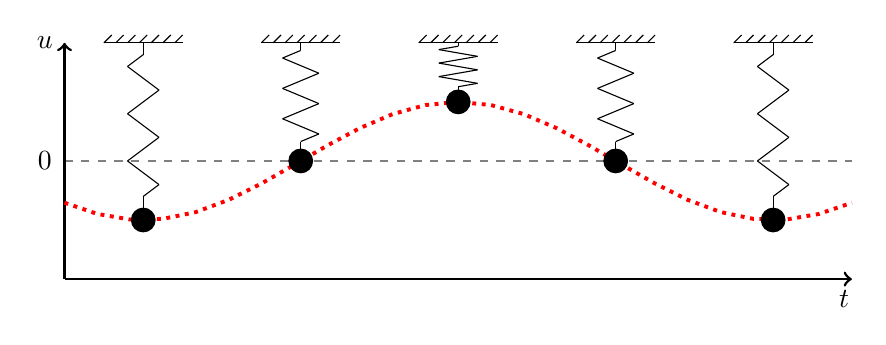
\begin{tikzpicture}
        
        \def\axisLineWidth{0.07};
            
        \def\zigzagLength{0.5}
        \def\zigzags{4}
        \pgfmathsetmacro\halfZigzags{\zigzags/2}
        \def\massSize{0.15}
        \def\massDistanceScaling{2}
        \def\amplitude{0.75}
        
        % axes
        \def\axisOffset{1}
        \draw[dashed, color = gray] (-\axisOffset, 0) -- (4*\massDistanceScaling+\axisOffset, 0);
        \node at (-\axisOffset-0.25, 1.5) {$u$};
        
        %u-axis
        \draw[->, line width=1] (-\axisOffset, -1.5) -- (-\axisOffset, 1.5);

        \node at (-\axisOffset - 0.25, 0) {$0$};

        %t-axis
        \draw[->, line width=1] (-\axisOffset, -1.5) -- (4*\massDistanceScaling+\axisOffset, -1.5);
        
        \node at (4*\massDistanceScaling + \axisOffset-0.1, -1.75) {$t$};

        % sine wave
        \draw[xshift=0 cm, xscale=4, domain=-0.25:2.25, dotted, variable=\x, red, line width=0.05cm] plot ({\x}, {-\amplitude*cos(180*\x)});

        \def\wallHeight{1.5}
        \def\wallHalf{0.5};
        \def\wallLineSpacing{0.15}
        \pgfmathsetmacro\halfNumDiag{\wallHalf / \wallLineSpacing}
        
        \foreach \massNo in {0, ..., 4}
        {
            \def\xshift{\massNo * \massDistanceScaling}

            \begin{scope}[xshift=\xshift cm]
                % draw wall
                \draw[-] (-\wallHalf, \wallHeight) -- (\wallHalf, \wallHeight) node[below, midway] (top) {};
                \foreach \bowDiag in {-\halfNumDiag, ...,\halfNumDiag}
                {
                    \draw[-] (\bowDiag * \wallLineSpacing, \wallHeight) -- (\bowDiag * \wallLineSpacing + 0.1, \wallHeight + 0.1);
                }
                
                \begin{scope}[yshift=1.5cm, rotate=180]
                    %spring extension
                    \pgfmathsetmacro\springHeight{1.5 + \amplitude*cos(\massNo * 90)}
    ;    
                    %what is the step in y
                    \pgfmathsetmacro\yInc{
                        (\springHeight-\massSize)/(2*(\zigzags+1)+4)
                    }

                    %what is the width of the spring based on its extension
                    \pgfmathsetmacro\halfSpringWidth{
                        0.5 * sqrt(\zigzagLength * \zigzagLength - 4 * \yInc * \yInc)
                    }

                    %small dot
                    \filldraw[black] (0, 0) circle (0pt) node[anchor=center](bottomSpring){};    

                    %start of spring
                    \draw[-] (0, 0) -- (0, \yInc);
                    \draw[-] (0, \yInc) -- (\halfSpringWidth, 2*\yInc);

                    % main zig zag
                    \def\curY{2*\yInc};
                    \def\curX{\halfSpringWidth};

                    \foreach \zig in {0, ...,\zigzags}
                    {
                        \pgfmathsetmacro\yToGoTo{\curY+2*\yInc};
                        % \filldraw[black] (0, \yToGoTo) circle (1pt) node[anchor=center](topSpring){\curX};           
                        \draw[-] (\curX, \curY) -- (-\curX, \yToGoTo);
                        \pgfmathsetmacro\tmpX{-\curX};

                        \global\let\curX=\tmpX;
                        \global\let\curY=\yToGoTo;
                    }

                    %end of spring
                    \pgfmathsetmacro\yToGoTo{\curY+\yInc};
                    \draw[-] (\curX, \curY) -- (0, \yToGoTo);
                    \global\let\curY=\yToGoTo;
                    \pgfmathsetmacro\yToGoTo{\curY+\yInc};
                    \draw[-] (0, \curY) -- (0, \yToGoTo);

                    %mass
                    \filldraw[black] (0, \yToGoTo+\massSize) circle (\massSize) node[anchor=center](topSpring){};   
                \end{scope}
            \end{scope}
        }
        % \node at (-0.5, 0.75) (K) {$K$};

    \end{tikzpicture}
    \caption{Mass-spring system over time. The system follows a harmonic (sinusoidal) motion. \label{fig:massSpring}}
\end{figure}